\subsection*{הקדמה}

נתחיל עם קצת רקע: החוברת הזאת היא חוברת עם מנגינות לנגינה על כלי פריטה קטנטן שנקרא „אוּקוּלֶלֶה” (השם הזה, \L{{\fontspec{Gentium}ʻ}ukulele}, מגיע משפה שנקראת הוואיאית; המשמעות שלו היא „פרעוש קופץ”). החוברת מיועדת למתחילים, מה שמתבטא בכמה אופנים:
\begin{compactitem}
	\item בחירה במנגינות מוכרות, חלקן שירים ידועים בעברית. לא כולן בהכרח „הלחם והטחינה” של כולם, אבל אני די בטוח שלפחות את חלקן תזהו.
	\item החוברת כוללת את הקו המלודי של המנגינות, ולא ליווי באקורדים, שהם לא שקופים להבנה.
	\item עיבדתי את המנגינות כך שבכל רגע נתון פורטים רק על מיתר אחד (מונופוניה). אחרי שתתאמנו על כל המנגינות שבחוברת תהיו מוכנים לגמרי לנגן כמה קולות (פוליפוניה).
	\item את הקטעים הקלאסיים קיצרתי ופישטתי.
	\item אופן ההצגה: בנוסף לסימון תווים בשיטה המערבית הרגילה לפי גובה הצליל, מצורפת טבלטורה. הטבלטורה מסמנת בדיוק על איזה סריג ללחוץ ועל איזה מיתר לפרוט (ולכן היא מתאימה לאוקוללה לפי הכיוון הרגיל בלבד, ולא לכלים אחרים). באופן כזה, כשהתווים הרגילים והטבלטורה נמצאים אחד מעל השני, מי שיודעים לקרוא תווים יכולים לקרוא גם אותם (ולנגן לפיהם בכלי־נגינה אחרים), וכולם יכולים לנגן לפי הטבלטורה.
\end{compactitem}
רמת הקושי של הנעימות לא אחידה, ובמתכוון הן מעורבבות.



\subsection*{כיוון}

\begin{wrapfigure}[5]{l}{3.5cm}\vspace{-\baselineskip}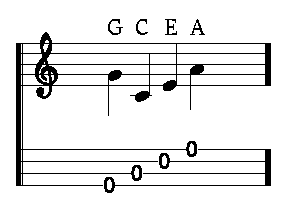
\includegraphics[width=3cm]{agordo.eps}\end{wrapfigure}
לאוקוללה ארבעה מיתרים. הם מכוונים באופן קצת מוזר: לא לפי גובה הצליל כמו ברוב כלי המיתר, אלא בסדר אחר~— המיתר הראשון\footnote{הגבוה ביותר כשאתם מחזיקים את האוקוללה בנגינה; הנמוך ביותר בטבלטורה.} מכוון בכיוון הרגיל לסול (\L{G}), הבא בתור לדו (\L{C}) באותה האוקטבה, ולאחריהם מי (\L{E}) ולה (\L{A}). ככה:

הדרך הכי קלה לכוון את האוקוללה היא בעזרת מכשיר כיוון אלקטרוני שמצמידים בתופסן לקצה הכלי: הוא חש את הרעידות ומתרגם אותן לסימון של גובה הצליל. חשוב שתשיגו מכוון שלא מותאם לגיטרה בלבד אלא כזה שהוא כללי.



\subsection*{איך קוראים טבלטורה?}

נכון שלאוקוללה יש ארבעה מיתרים? אז לטבלטורה יש ארבע שורות, שמייצגות את ארבעת המיתרים (כאילו היא אוקוללה שמונח עם הראש בצד שמאל). ימניים פורטים עם יד ימין ולוחצים בין הסריגים ביד שמאל.

קוראים את הטבלטורה לפי הסדר, משמאל לימין, וכשיש מספר אז לוחצים בין הסריגים במיתר המתאים ופורטים עליו: 0 מסמן פריטה על מיתר פתוח, בלי ללחוץ ביד השניה; 1 מסמן ללחוץ על המיתר לפני הסריג הראשון ולפרוט עליו; 2 לפני הסריג השני, וכן הלאה. בדרך־כלל יש סימונים על האוקוללה שמטרתם לעזור למצוא בקלות את הסריגים הרחוקים יותר. הנה שלוש דוגמאות לנגינה של שלושה צלילים:

\vspace{\baselineskip}
\begin{minipage}{4cm}
	\centering
	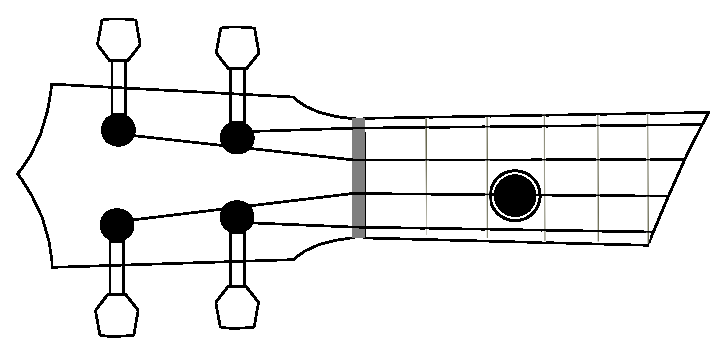
\includegraphics[width=3cm]{plano-C3.eps}\\
	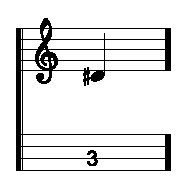
\includegraphics[height=2.5cm]{tab-C3.eps}
\end{minipage}\hfill
\begin{minipage}{4cm}
	\centering
	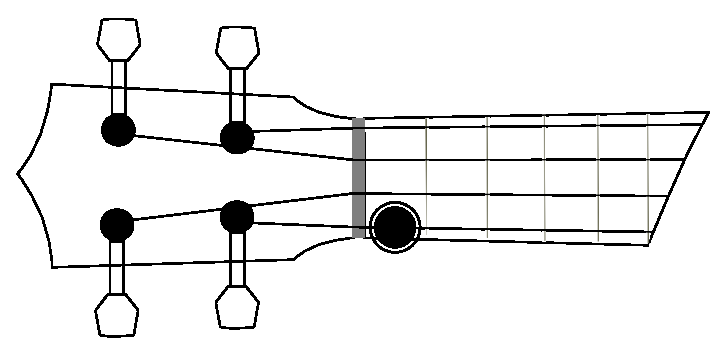
\includegraphics[width=3cm]{plano-G1.eps}\\
	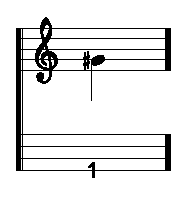
\includegraphics[height=2.5cm]{tab-G1.eps}
\end{minipage}\hfill
\begin{minipage}{4cm}
	\centering
	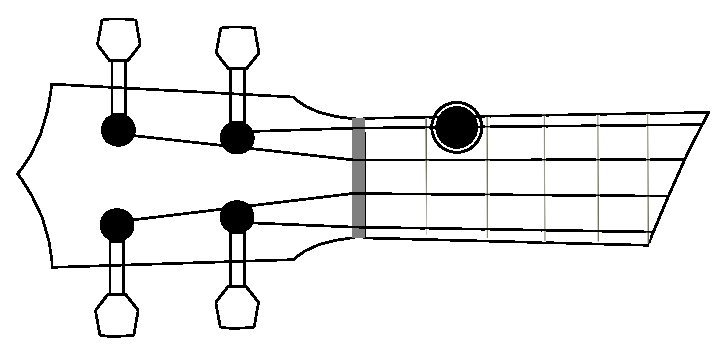
\includegraphics[width=3cm]{plano-A2.eps}\\
	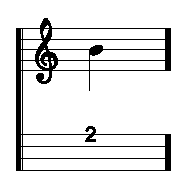
\includegraphics[height=2.5cm]{tab-A2.eps}
\end{minipage}
\vspace{\baselineskip}

הסימון של משך הצליל מצויין אצלנו רק בתווים, באופן רגיל: \symbolglyph{𝅝} מסמן משך שלם (\L{1}), \symbolglyph{𝅗𝅥} מסמן חצי (\L{½}), \symbolglyph{𝅘𝅥} מסמן רבע (\L{¼}), ו־\symbolglyph{𝅘𝅥𝅮} או \symbolglyph{♫} מסמנים שמינית (\L{⅛}); המקבילות של ההפסקות הן \symbolglyph{𝄻}, \symbolglyph{𝄼}, \symbolglyph{𝄽} ו־\symbolglyph{𝄾}, בהתאמה.

רוצים לוודא שהבנתם? הנה ההתחלה של „יונתן הקטן”. תנסו לראות אם זה אכן מה שיוצא לכם כשאתם מנגנים:

\begin{center}
	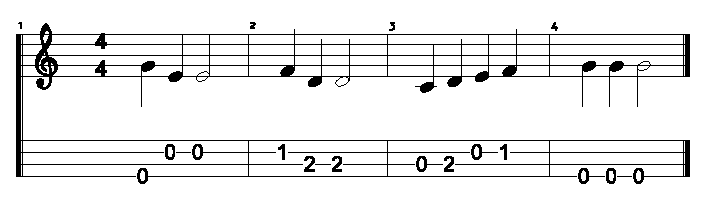
\includegraphics[height=2.5cm]{jon.eps}
\end{center}

חזרות מסומנות ב־\symbolglyph{𝄆} ו־\symbolglyph{𝄇}. כשיש הבדל בין החזרה הראשונה והשניה משמש סימון \symbolglyph{⌜} ממוספר מעל התיבות השונות.

\subsection*{מידע נוסף ויצירת קשר}

\begin{wrapfigure}[4]{l}{1.75cm}\vspace{-\baselineskip}
\includegraphics[width=1.5cm]{retejo.png}\end{wrapfigure}
האתר של החוברת הוא \url{http://xpr.digitalwords.net/ukulele}; בקוד \L{QR}:

באתר נמצאים כל קבצי המקור של החוברת, כמו גם קובץ מוכן להדפסה (אם תרצו ליצור עותק נוסף או לקרוא במחשב). את הטבלטורות הכנתי בעזרת התוכנה החופשית \L{TuxGuitar}; היא זמינה להורדה בכתובת \url{http://tuxguitar.com.ar}. אם תפתחו את קבצי המקור של המנגינות (סיומת \texttt{.tg}) בתוכנה הזאת תוכלו לשמוע אותן כשבזמן אמת מסומן המקום המתאים בטבלטורה ואופן הנגינה על ציור סכימטי של אוקוללה.

החוברת הזאת חופשית (נחלת הכלל, \L{public domain}): אתם יכולים להעתיק, לשנות, להפיץ ולהשתמש בה כרצונכם.

בכל עניין, אל תהססו לפנות אלי בדואל (\url{ukulele@digitalwords.net}) או בטלפון (02-6419913).

\vspace{\baselineskip}
~\hfill
\begin{minipage}{3cm}
	יודה רונן\\
	ירושלים 2014\\
\end{minipage}
